\part{高等数学}

% \newcounter{counter1}
% \addtocounter{counter1}{1}
% \renewcommand{\thesubsection}{\arabic{section}}
% \setcounter{counter1}{}

开始于2023年3月1日\\高昆轮\\
林德松

\chapter*{常用基础知识}
\addcontentsline{toc}{chapter}{常用基础知识}
\subsubsection{数列}
\begin{enumerate}
\item 等差数列\par
首项为$ a_{1} $,公差为$ d(d\neq 0) $的数列$ a_{1},a_{1}+d,a_{1}+2d,...,a_{1}+(n-1)d,... $.
\begin{enumerate}
\item 通项公式: $ a_{n}=a_{1}+(n-1)d $
\item 前$ n $项的和: $ S_{n}=\frac{n}{2}(a_{1}+a_{n})=\frac{n}{2}[2a_{1}+(n-1)d] $
\end{enumerate}
\item 等比数列\par
首项为$ a_{1} $, 公比为$ r(r\neq 0) $的数列$ a_{1},a_{1}r,...,a_{1}r^{n-1},... $.
\begin{enumerate}
\item 通项公式: $ a_{n}=a_{1}r^{n-1} $
\item 前$ n $项的和$ S_{n}=\scaleleftright[6pt]{\biggl\{}{\begin{aligned}
& na_{1}\ & r=1 \\
& \frac{a_{1}(1-r^{n})}{1-r} & r\neq 1
\end{aligned}}{.} $
\item 一些常见数列前$ n $项的和\par
\begin{enumerate}
\item $ \sum_{k=1}^{n}k=1+2+3+...+n=\frac{n(1+n)}{2} $
\item $ \sum_{k=1}^{n}k^{2}=1^{2}+2^{2}+...+n^{2}=\frac{n(n+1)(2n+1)}{6} $
\item $ \sum_{k=1}^{n}\frac{1}{k(k+1)}=\frac{1}{1\times 2}+\frac{1}{2\times 3}+...+\frac{1}{n(n+1)}=\frac{n}{n+1} $
\end{enumerate}
\end{enumerate}
\end{enumerate}
\subsubsection{三角函数}
\begin{enumerate}
\item 三角函数的基本关系
\[ \begin{split}&\csc \alpha=\frac{1}{\sin \alpha},\ \sec \alpha=\frac{1}{\cos \alpha},\ \cot \alpha=\frac{1}{\tan \alpha}\\& \sin^{2}\alpha +\cos^{2}\alpha =1,\ 1+\tan^{2}\alpha = \sec^{2}\alpha,\ 1+\cot^{2}\alpha =\csc^{2}\alpha\\ &\tan \alpha=\frac{\sin \alpha}{\cos \alpha},\ \cot \alpha=\frac{\cos \alpha}{\sin \alpha}\end{split}\]
\item 重要公式
\item 倍角公式
\[ \begin{split}
& \sin 2\alpha=2\sin \alpha \cos \alpha,\ \cos 2\alpha =\cos^{2}\alpha -\sin^{2}\alpha =1-2\sin^{2}\alpha\\&=2\cos^{2}\alpha -1,\ \tan 2\alpha =\frac{2\tan \alpha}{1-\tan^{2}\alpha}
\end{split} \]
\item 半角公式
\[ \begin{split}
& \sin^{2}\frac{\alpha}{2}=\frac{1}{2}(1-\cos \alpha),\ \cos^{2}\frac{\alpha}{2}=\frac{1}{2}(1+\cos \alpha) \\
& \tan \frac{\alpha}{2}=\frac{1-\cos \alpha}{\sin \alpha}=\frac{\sin \alpha}{1+\cos \alpha}=\pm \sqrt{\frac{1-\cos \alpha}{1+\cos \alpha}}
\end{split} \]
\item 和差公式
\[ \begin{split}
& \sin(\alpha \pm \beta)=\sin\alpha\cos\beta \pm \cos\alpha\sin\beta \\
& \cos(\alpha \pm \beta)=\cos\alpha\cos\beta \mp \sin\alpha\sin\beta \\
& \tan(\alpha \pm \beta)=\frac{\tan\alpha \pm \tan\beta}{1 \mp \tan\alpha\tan\beta}
\end{split} \]
\item 积化和差公式
\[ \begin{split}
& \sin\alpha\cos\beta = \frac{1}{2}[\sin(\alpha + \beta) + \sin(\alpha - \beta)] \\
& \cos\alpha\sin\beta = \frac{1}{2}[\sin(\alpha + \beta) - \sin(\alpha - \beta)] \\
& \cos\alpha\cos\beta = \frac{1}{2}[\cos(\alpha + \beta) + \cos(\alpha - \beta)] \\
& \sin\alpha\sin\beta = -\frac{1}{2}[\cos(\alpha + \beta) - \cos(\alpha - \beta)] \\
\end{split} \]
\item 和差化积公式
\[ \begin{split}
& \sin\alpha + \sin\beta = 2\sin\frac{\alpha+\beta}{2}\cos\frac{\alpha - \beta}{2} \\
& \sin\alpha - \sin\beta = 2\cos\frac{\alpha+\beta}{2}\sin\frac{\alpha - \beta}{2} \\
& \cos\alpha + \cos\beta = 2\cos\frac{\alpha+\beta}{2}\cos\frac{\alpha - \beta}{2} \\
& \cos\alpha - \cos\beta = -2\sin\frac{\alpha+\beta}{2}\sin\frac{\alpha - \beta}{2} \\
\end{split} \]
\item 万能公式\par
若$ u=\tan \frac{x}{2}(-\pi<x<\pi) $, 则$ \displaystyle\hspace{.2em}\sin x=\frac{2u}{1+u^{2}} $, $ \displaystyle\hspace{.2em}\cos x=\frac{1-u^{2}}{1+u^{2}} $.
\end{enumerate}
\subsubsection{指数运算法则}
\vspace*{-2em}
\[ \begin{split}
& a^{\alpha}\cdot a^{\beta}=a^{\alpha + \beta},\  \frac{a^{\alpha}}{a^{\beta}}=a^{\alpha-\beta} \\
& (a^{\alpha})^{\beta}=a^{\alpha \beta},\ (ab)^{\alpha}=a^{\alpha}b^{\alpha},\ (\frac{a}{b})^{\alpha}=\frac{a^{\alpha}}{b^{\alpha}}
\end{split} \]
\subsubsection{对数运算法则}
\begin{enumerate}
\item $ \log_{a}(MN)=\log_{a}M+\log_{a}N  $
\item $ \log_{a}\frac{M}{N}=\log_{a}M-\log_{a}N $
\item $ \log_{a}^{n}=n\log_{a}M $
\item $ \log_{a}\sqrt[n]{M}=\frac{1}{n}\log_{a}M $
\end{enumerate}
\subsubsection{一元二次方程基础}
\begin{enumerate}
\item 一元二次方程: $ ax^{2}+bx+c=0(a\neq 0) $
\item 根的公式: $ x_{1,2}=\frac{-b\pm \sqrt{b^{2}-4ac}}{2a} $
\item 根和系数的关系: $ x_{1}+x_{2}=-\frac{b}{a},\ x_{1}x_{2}=\frac{c}{a} $
\item 判别式: $ \Delta=b^{2}-4ac $
\item 抛物线定点坐标: $ (-\frac{b}{2a},c-\frac{b^{2}}{4a}) $
\end{enumerate}
\subsubsection{因式分解公式}
\begin{enumerate}
\item $ (a+b)^{2}=a^{2}+b^{2}+2ab $
\item $ (a-b)^{2}=a^{2}+b^{2}-2ab $
\item $ (a+b)^{3}=a^{3}+3a^{2}b+3b^{2}a+b^{3} $
\item $ (a-b)^{3}=a^{3}-3a^{2}b+3b^{2}a-b^{3} $
\item $ a^{3}+b^{3}=(a+b)(a^{2}-ab+b^{2}) $
\item $ a^{3}-b^{3}=(a-b)(a^{2}+ab+b^{2}) $
\item $ a^{2}-b^{2}=(a+b)(a-b) $
\item 二项式定理: $ (a+b)^{n}=\sum_{k=0}^{n}C_{n}^{k}a^{n-k}b^{k} $
\end{enumerate}
\subsubsection{阶乘和双阶乘}
\begin{enumerate}
\item $ n!=1\cdot 2\cdot 3\cdot ... \cdot n $, 规定$ 0!=1 $
\item $ (2n)!!=2\cdot 4\cdot 6\cdot ... \cdot (2n)=2^{n}n! $
\item $ 2(n-1)!!=1\cdot 3\cdot 5\cdot ... \cdot (2n-1) $
\end{enumerate}
\subsubsection{常用不等式}
\begin{enumerate}
\item 设$ a,b $为实数, 则有:
\begin{enumerate}
\item $ |a\pm b|\le |a|+|b| $
\item $ ||a|-|b||\le |a-b| $
\end{enumerate}
\item $ \sqrt{ab}\le \frac{a+b}{2}\le \sqrt{\frac{a^{2}+b^{2}}{2}}(a,b>0) $
\item 设$ a>b>0 $, 则$ \scaleleftright[6pt]{\biggl\{}{\begin{aligned}
& \text{当}n>0\text{时}, a^{n}>b^{n} \\
& \text{当}n<0\text{时}, a^{n}<b^{n}
\end{aligned}}{.} $
\item 若$ 0<a<x<b,0<c<y<d $, 则$ \frac{c}{b}<\frac{y}{x}<\frac{d}{a} $
\item $ \sin x<x<\tan x(0<x<\frac{\pi}{2}) $
\item $ \sin x<x(x>0) $
\item $ \arctan x\le x\le \arcsin x(0\le x\le 1)$
\item $ e^{x}\ge x+1(\forall x) $
\item $ x-1\ge \ln x(x>0) $
\item $ \frac{1}{1+x}<\ln (1+\frac{1}{x})<\frac{1}{x}(x>0) $
\end{enumerate}


\chapter{函数极限连续}
\section{考点1 常用函数及常用曲线p4}
\subsection{函数的概念及一些常用函数}
\begin{enumerate}
    \item 常见函数
    \begin{enumerate}
        \item 常数函数\par
        $ y=C $, $ C $为常数, 图形为平行于$ x $轴的水平直线.
        \item 幂函数\par
        $ y=x^{\mu} $\ ($ \mu $是实数)
        \begin{tcolorbox}
        \begin{enumerate}
        \item 见到$ \sqrt{u},\sqrt[3]{u} $, 用$ u $来研究最值
        \item 见到$ |u| $时, 用$ u^{2} $来研究最值
        \item 见到$ u_{1}u_{2}u_{3} $时, 用$ ln(u_{1}u_{2}u_{3})=lnu_{1}+lnu_{2}+lnu_{3} $来研究最值
        \item 见到$ \frac{1}{u} $时, 用$ u $来研究最值
        \end{enumerate}
        \end{tcolorbox}
        \item 指数函数
        $ y=a^{x} $\ ($ a>0,a\neq 1 $)
        \item 对数函数
        $ y=log_{a}x $\ ($ a>0,a\neq 1 $)
        \begin{tcolorbox}
        常用公式: $ x=e^{lnx}\ (x>0), u^{v}=e^{lnu^{v}}=e^{vlnu}\ (u>0) $
        \end{tcolorbox}
        \item 三角函数
    \end{enumerate}
    \item 绝对值函数\\
    y=|x|在x=0处连续,但是是不可导的(左导数不等于右导数)\par
        \begin{equation*}
        y=|x|=
        \scaleleftright[6pt]{\biggl\{}{
        \begin{aligned}
        & x,\ x\ge 0 \\
        & -x,\ x<0
        \end{aligned}
        }{.}
        \end{equation*}
    \pmb{重要公式}$|a_1 \pm a_2 \pm... \pm a_n|\le|a_1|+|a_2|+...+|a_n|$

    \item 最值函数\\
    $\displaystyle\hspace{.2em} U=max\{f(x),g(x)\}= \frac{f(x)+g(x)+|f(x)-g(x)|}{2}$\\
    $\displaystyle\hspace{.2em} V=min\{f(x),g(x)\}= \frac{f(x)+g(x)-|f(x)-g(x)|}{2}$\\
    $U+V=f(x)+g(x),U-V=|f(x)-g(x)|,U \cdot V=f(x)g(x)$

    \item 符号函数\\
    对任何$x$,都有$\sqrt{x^2}=|x|=xsgn(x)$\par
    \begin{equation*}
        y=\text{sgn}\ x=
        \scaleleftright[6pt]{\biggl\{}{
            \begin{aligned}
                & 1,\ x>0 \\
                & 0,\ x=0 \\
                & -1,\ x<0
            \end{aligned}
            }{.}
        \end{equation*}
    
    \item 取整函数\\
    $[x+n]=[x]+n,其中n是整数,x-1<[x]\le x $
    
    \item 幂指函数\\
    $\displaystyle\hspace{.2em} u(x)^{v(x)}=e^{v(x)lnu(x)}$
    
    \item 狄利克雷函数
    {
        % \begin{equation}
        $D(x)=\left\{
            \begin{array}{cl}
                1,&x\in Q\\
                0,&x\in Q^C\\
            \end{array}
            \right.$
        % \end{equation}
    }
\end{enumerate}



\subsection{反函数、复合函数及初等函数}
\begin{enumerate}
    \item 反函数
    \begin{enumerate}
        \item $y=\sin x$的反函数\\
        当$0\le x\le \frac{\pi}{2}$时,$x=\arcsin y,y\in [0,1]$\\
        当$\frac{\pi}{2}\le x\le \frac{3\pi}{2}$时,$x=\pi -\arcsin y,y\in [-1,1)$\\
        当$\frac{3\pi}{2}\le x\le 2\pi$时,$x=2\pi +\arcsin y,y\in (-1,0]$
    \end{enumerate}
    \item 复合函数
    \item 初等函数
    \begin{enumerate}
        \item 反对幂三指
        \item 幂指函数是初等函数
        \item 三角函数
            \begin{enumerate}
            \item 正弦函数和余弦函数\par
            正弦函数$ y=\sin x $, 余弦函数$ y=\cos x $.
            \item 正切函数和余切函数\par
            正切函数$ y=\tan x $, 余切函数$ y=\cot x $.\par
            \begin{figure}[H]
            \centering
            \begin{subfigure}{.475\linewidth}
            \centering
            \begin{tikzpicture}[
            ]
            \begin{axis}[
            width=\linewidth,
            axis lines=middle,
            xmin=-4.3,
            xmax=4.3,
            ymin=-4.5,
            ymax=4.5,
            xlabel=$ x $,
            ylabel=$ y $,
            xlabel=$ x $,
            xlabel style={below},
            ylabel=$ y $,
            ylabel style={left},
            xtick={-pi/2,pi/2},
            xticklabels={$ -\frac{\pi}{2} $,$ \frac{\pi}{2} $},
            xticklabel style={left,yshift=-0.5em},
            ytick={1},
            yticklabels={$ 1 $},
            extra y ticks={-1},
            extra y tick labels={$ -1 $},
            extra y tick style={tick label style={right,yshift=-1em}},
            ]
            \addplot [black,samples=1000]{tan(deg(x))};
            \end{axis}
            \end{tikzpicture}
            \caption{正切函数图像}
            \end{subfigure}
            \hspace{.1em}
            \begin{subfigure}{.475\linewidth}
            \centering
            \begin{tikzpicture}[
            ]
            \begin{axis}[
            width=\linewidth,
            axis lines=middle,
            xmin=-4.3,
            xmax=4.3,
            ymin=-4.5,
            ymax=4.5,
            xlabel=$ x $,
            xlabel style={below},
            ylabel=$ y $,
            ylabel style={left},
            xtick={-pi/2,pi/2},
            xticklabels={$ -\frac{\pi}{2} $,$ \frac{\pi}{2} $},
            xticklabel style={left,yshift=-0.5em},
            ytick={1},
            yticklabels={$ 1 $},
            extra y ticks={-1},
            extra y tick labels={$ -1 $},
            extra y tick style={tick label style={right,yshift=-1em}},
            ]
            \addplot [black,samples=1000]{1/tan(deg(x))};
            \end{axis}
            \end{tikzpicture}
            \caption{余切函数图像}
            \end{subfigure}
            \end{figure}
            \item 正割函数和余割函数\par
            正割函数$ y=\sec x $, 余割函数$ y=\csc x $.
            \begin{figure}[H]
            \centering
            \begin{subfigure}{.475\linewidth}
            \centering
            \begin{tikzpicture}[
            ]
            \begin{axis}[
            width=\linewidth,
            axis lines=middle,
            xmin=-4.3,
            xmax=4.3,
            ymin=-4.5,
            ymax=4.5,
            xlabel=$ x $,
            ylabel=$ y $,
            xtick={-pi/2,pi/2},
            xticklabels={$ -\frac{\pi}{2} $,$ \frac{\pi}{2} $},
            xticklabel style={left,yshift=-0.5em},
            ytick={-1,1},
            yticklabels={$ -1 $,$ 1 $},
            yticklabel style={below,xshift=-1em,yshift=0.4em},
            ]
            \addplot [black,samples=1000]{1/cos(deg(x))};
            \end{axis}
            \end{tikzpicture}
            \caption{正割函数图像}
            \end{subfigure}
            \begin{subfigure}{.475\linewidth}
            \begin{tikzpicture}[
            ]
            \begin{axis}[
            width=\linewidth,
            axis lines=middle,
            xmin=-4.3,
            xmax=4.3,
            ymin=-4.5,
            ymax=4.5,
            xlabel=$ x $,
            ylabel=$ y $,
            ylabel style={left},
            xtick={pi/2},
            xticklabels={$ \frac{\pi}{2} $},
            extra x ticks={-pi/2},
            extra x tick labels={$ -\frac{\pi}{2} $},
            extra x tick style={tick label style={above}},
            ytick={1},
            yticklabels={$ 1 $},
            extra y ticks={-1},
            extra y tick labels={$ -1 $},
            extra y tick style={tick label style={right,yshift=-0.5em}},
            ]
            \addplot [black,samples=1000]{1/sin(deg(x))};
            \end{axis}
            \end{tikzpicture}
            \caption{余割函数图像}
            \end{subfigure}
            \end{figure}
            \end{enumerate}
        \item 反三角函数
            \begin{enumerate}
            \item 反正弦函数和反余弦函数\par
            反正弦函数$ y=\arcsin x $, 反余弦函数$ y=\arccos x $.
            \begin{figure}[H]
            \centering
            \begin{subfigure}{.475\linewidth}
            \centering
            \begin{tikzpicture}[
            ]
            \begin{axis}[
            width=\linewidth,
            axis lines=middle,
            domain=-1:1,
            xmin=-2,
            xmax=2,
            ymin=-2,
            ymax=2,
            xlabel=$ x $,
            ylabel=$ y $,
            xtick={-1,1},
            ytick={-pi/2,pi/2},
            yticklabels={$ -\frac{\pi}{2} $, $ \frac{\pi}{2} $},
            ]
            \addplot [black,samples=1000]{asin(x)/180*pi};
            \end{axis}
            \end{tikzpicture}
            \caption{反正弦函数图像}
            \end{subfigure}
            \begin{subfigure}{.475\linewidth}
            \begin{tikzpicture}[
            ]
            \begin{axis}[
            width=\linewidth,
            axis lines=middle,
            domain=-1:1,
            xmin=-2,
            xmax=2,
            ymin=-0.5,
            ymax=4,
            xlabel=$ x $,
            ylabel=$ y $,
            ytick={pi/2,pi},
            yticklabels={$ \frac{\pi}{2} $, $ \pi $},
            xtick={-1,1},
            xticklabels={$ -1 $,$ 1 $},
            ]
            \addplot [black,samples=1000]{acos(x)/180*pi};
            \end{axis}
            \end{tikzpicture}
            \caption{反余弦函数图像}
            \end{subfigure}
            \end{figure}
            \item 反正切函数和反余切函数\par
            反正切函数$ y=\arctan x $, 反余切函数$ y=\arccot x $
            \begin{figure}[H]
            \centering
            \begin{subfigure}{.475\linewidth}
            \centering
            \begin{tikzpicture}[
            ]
            \begin{axis}[
            width=\linewidth,
            axis lines=middle,
            xmin=-2,
            xmax=2,
            ymin=-2,
            ymax=2,
            xlabel=$ x $,
            ylabel=$ y $,
            xtick={\empty},
            ytick={-pi/2,pi/2},
            yticklabels={$ -\frac{\pi}{2} $, $ \frac{\pi}{2} $},
            ]
            \addplot [black,samples=1000]{atan(x)/180*pi};
            \end{axis}
            \end{tikzpicture}
            \caption{反正切函数图像}
            \end{subfigure}
            \begin{subfigure}{.475\linewidth}
            \begin{tikzpicture}[
            ]
            \begin{axis}[
            width=\linewidth,
            axis lines=middle,
            xmin=-2,
            xmax=2,
            ymin=-0.5,
            ymax=4,
            xlabel=$ x $,
            ylabel=$ y $,
            ytick={pi/2,pi},
            yticklabels={$ \frac{\pi}{2} $, $ \pi $},
            xtick={\empty},
            ]
            \addplot [black,samples=1000]{(pi/2)-(atan(x))/180*pi};
            \end{axis}
            \end{tikzpicture}
            \caption{反余切函数图像}
            \end{subfigure}
            \end{figure}
            \end{enumerate}
    \end{enumerate}


\end{enumerate}

\subsection{函数表达式的求解}

\begin{enumerate}
    \item 一般借助微分方程(第八章)求解
    \item 注意$\lim \limits_{x\to x_0}f(x),f'(x_0),\int_{a}^{b}f(x)dx$等都是一个数
    \item 抓大头
    \begin{tcolorbox}
        \pmb{重要公式}\newline
        $\displaystyle\hspace{.2em}\lim \limits_{n\to \infty}\sqrt{a_1^n+a_2^n+...+a_m^n}=max\{a_1,a_2,...,a_m\}$\\
        \hyperref[考点12例六]{考点12例六}
    \end{tcolorbox}

\end{enumerate}

\subsection{常用曲线(这些曲线在以后会经常碰到)}

\begin{enumerate}
    \item 笛卡尔心形线\\
    $x^2+y^2=a(\sqrt[]{x^2+y^2}-x)$或$r=a(1-\cos \theta)$(桃屁股朝右)\\
    $x^2+y^2=a(\sqrt[]{x^2+y^2}+x)$或$r=a(1+\cos \theta)$(桃屁股朝左)\\
    与$x$轴交点$O,\mp 2a$,与$y$轴交点$\pm a$\par
    $ r=a(1-\cos \theta)(a>0) $
    \begin{figure}[H]
        \centering
        \begin{tikzpicture}[
        >=stealth,
        ]
        \draw[->] (0,0)node[left]{$ 0 $} to (1,0)node[right]{$ x $};
        \draw[domain=0:360,samples=1000,scale=.7] plot (\x:{2*(1-cos(\x))});
        \end{tikzpicture}
        \caption{心形线}
    \end{figure}

    \item 玫瑰线\par
    $ r=a\sin 3\theta (a>0) $
    \begin{figure}[H]
        \centering
        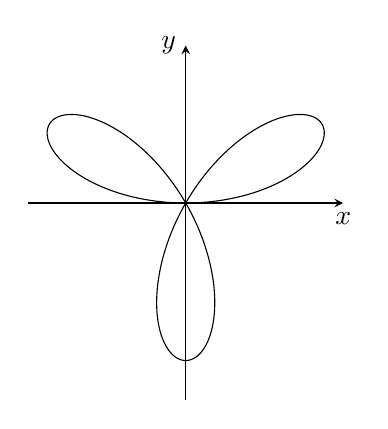
\begin{tikzpicture}[
        >=stealth,
        ]
        \draw[->] (-2,0) to (2,0)node[below]{$ x $};
        \draw[->] (0,-2.5) to (0,2)node[left]{$ y $};
        \draw[domain=0:360,samples=1000,scale=1] plot (\x:{2*sin(3*\x)});
        \end{tikzpicture}
        \caption{玫瑰线}
    \end{figure}
    
    \item 阿基米德螺线\par
    $ r=a\theta (a>0,\theta \ge 0) $
    \begin{figure}[H]
        \centering
        \begin{tikzpicture}[
        >=stealth,
        ]
        \draw[->] (0,0)node[left]{$ 0 $} to (3,0)node[below]{$ x $};
        \draw[domain=0:360,samples=1000,scale=.2] plot (\x:{2*(\x/180*pi)});
        \end{tikzpicture}
        \caption{阿基米德螺线}
    \end{figure}

    \item 伯努利双纽线\par
    $ r^{2}=a^{2}\cos 2\theta(a>0) $一二三四象限\\
    $ r^{2}=a^{2}\sin 2\theta(a>0) $一三象限.
    \begin{figure}[H]
        \centering
        \begin{subfigure}{.475\linewidth}
        \centering
        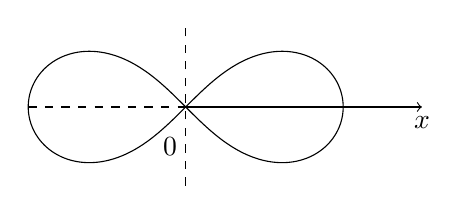
\begin{tikzpicture}
        \draw[->] (0,0) to (3,0)node[below]{$ x $};
        \node at (-.2,-.5){$ 0 $};
        \draw[dashed] (0,-1) to (0,1);
        \draw[dashed] (-2,0) to (0,0);
        \draw[domain=0:45,samples=1000] plot (\x:{sqrt(4*cos(2*\x))});
        \draw[domain=135:225,samples=1000] plot (\x:{sqrt(4*cos(2*\x))});
        \draw[domain=315:360,samples=1000] plot (\x:{sqrt(4*cos(2*\x))});
        \end{tikzpicture}
        \caption{$ r^{2}=a^{2}\cos 2\theta $}
        \end{subfigure}
        \hfill
        \begin{subfigure}{.475\linewidth}
        \centering
        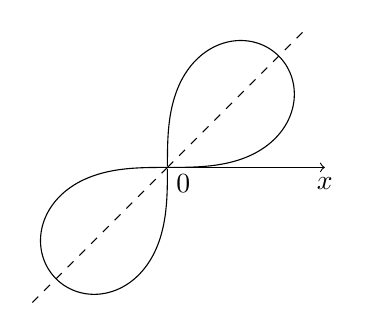
\begin{tikzpicture}
        \draw[->] (0,0) to (2,0)node[below]{$ x $};
        \node at (.2,-.2){$ 0 $};
        \draw[domain=0:90,samples=1000,] plot (\x:{sqrt(4*sin(2*\x))});
        \draw[domain=180:270,samples=1000,] plot (\x:{sqrt(4*sin(2*\x))});
        \draw[dashed] (0,0) to (45:2.5);
        \draw[dashed] (0,0) to (225:2.5);
        \end{tikzpicture}
        \caption{$ r^{2}=a^{2}\sin 2\theta $}
        \end{subfigure}
        \caption{伯努利双纽线}
    \end{figure}

    \item 摆线\par
    \begin{equation*}
        \scaleleftright[6pt]{\biggl\{}{
        \begin{aligned}
        & x=a(\theta-\sin \theta) \\
        & y=a(1-\cos \theta)
        \end{aligned}
        }{.}
    \end{equation*}
    \begin{figure}[H]
        \centering
        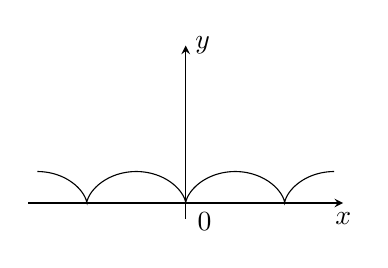
\begin{tikzpicture}[
        >=stealth,
        scale=2,
        ]
        \draw[->] (-1,0) to (1,0)node[below]{$ x $};
        \draw[->] (0,-.1) to (0,1)node[right]{$ y $};
        \node at (.12,-.12){$ 0 $};
        \draw[domain=-540:540][samples=1000] plot({(\x/180*pi-sin(\x))*0.1},{(1-cos(\x))*0.1});
        \end{tikzpicture}
        \caption{摆线}
    \end{figure}

    \item 星形线\par
    \begin{equation*}
        \scaleleftright[6pt]{\biggl\{}{
        \begin{aligned}
        & x=a\cos^{3}t \\
        & y=a\sin^{3}t
        \end{aligned}
        }{.}
    \end{equation*}
    \begin{figure}[H]
        \centering
        \begin{tikzpicture}[
        >=stealth,
        scale=2,
        ]
        \draw[->] (-1,0) to (1.2,0)node[below]{$ x $};
        \draw[->] (0,-1) to (0,1.2)node[right]{$ y $};
        \node at (.12,-.12){$ 0 $};
        \draw[domain=0:360][samples=1000] plot({(cos(\x))^3},{(sin(\x))^3});
        \end{tikzpicture}
        \caption{星形线}
    \end{figure}

    \item 笛卡尔叶形线\par
    {
        $  x^3+y^3-3axy=0$或$\left\{ \begin{array}{cl}
            \displaystyle\hspace{.2em}x=\frac{3at}{1+t^3},\\
            \displaystyle\hspace{.2em} y=\frac{3at^2}{1+t^3}
        \end{array}\right.$
    }\\
    渐近线$y=x$和$x+y=-a$
\end{enumerate}


\section{考点2 函数的几种特性(特别要记忆对这些特性总结的结论)p11}

\subsection{有界性}

\begin{enumerate}
    \item 有界无界应在具体区间判断
    \item 有界无界的判定方法\begin{enumerate}
        \item 用定义
        \item 用结论\\
        若$f(x)$在$[a,b]$上连续,则$f(x)$在$[a,b]$上有界\\
        若$f(x)$在$(a,b)$内连续,且$\lim \limits_{x\to a^+}f(x)$存在,$\lim \limits_{x\to b^-}f(x)$也存在,则$f(x)$在$(a,b)$内有界\\
        若存在$c\in I$,且$\lim \limits_{x\to c^-}f(x)=\infty$或$\lim \limits_{x\to c^+}f(x)=\infty$,则$f(x)$在区间$I$上无界
    \end{enumerate}
\end{enumerate}

\subsection{单调性}

\begin{enumerate}
    \item 判定方法\begin{enumerate}
        \item 用定义
        \item 用结论\\
        导数大于(小于)0,$f(x)$单调增加(减少)\\
        复合函数\underline{同增异减}
    \end{enumerate}
\end{enumerate}

\subsection{奇偶性}

\begin{enumerate}
    \item 常见的奇函数\begin{itemize}
        \item $x, \sin x, \tan x, sgn x$
        \item $\ln (x+\sqrt[]{1+x^2})$
        \item $\displaystyle\hspace{.2em}\frac{a^{kx}\pm 1}{a^{kx}\mp 1}$$(a>0$且$a \ne 1, k \ne 0)$
        \item \underline{$f(x)-f(-x)$}
    \end{itemize}
    \item 常见的偶函数\begin{itemize}
        \item $C, x^2, |x|, \cos x$
        \item \underline{$f(x)+f(-x)$}
    \end{itemize}
    \item 判定方法\begin{enumerate}
        \item 用定义
        \item 用结论\\    
        奇$\pm$奇=奇,偶$\pm$偶=偶,奇$\cdot$奇=奇=偶,偶$\cdot$偶=偶,奇$\cdot$偶=奇\\
        \underline{内偶则偶,内奇看外},外奇则奇,外偶则偶\\
        
        若$f(x)$是\underline{可导}的奇(偶)函数,则$f'(x)$是偶(奇)函数\\
        若$f(x)$是\underline{连续}的奇(偶)函数,则$\int_{0}^{x}f(t)dt$是偶(奇)函数(下限必须为0)
    \end{enumerate}
\end{enumerate}

\subsection{周期性}

\begin{enumerate}
    \item 判定方法\begin{enumerate}
        \item 用定义
        \item 用结论\begin{enumerate}
            \item 若$f(x)$以T为周期,则$f(ax+b)$以$\displaystyle\hspace{.2em}\frac{T}{|a|}$为周期
            \item 若$g(x)$是周期函数,则复合函数$f[g(x)]$也是周期函数
            \item 若$f(x)$是以T为周期的可导函数,则$f'(x)$也以T周期函数
            \item 若$f(x)$是以T为周期的连续函数,则只有在$\displaystyle\hspace{.2em}\int_{0}^{T}f(x)dx=0$时,$\displaystyle\hspace{.2em}\int_{a}^{x}f(t)dt$也以T周期函数
        \end{enumerate}
    \end{enumerate}
    \item 定义域关于原点对称的任一函数必可表示为一个偶函数与一个奇函数之和
\end{enumerate}

\section{考点3 极限的定义p14}

\section{考点4 极限的性质p19}

\section{考点5 无穷小与无穷大p20}

\section{考点6 极限的四则运算法则及两个重要极限p25}

\subsection{极限的四则运算法则}

\begin{enumerate}
    \item 若$\lim f(x)=A (\exists)$,$\lim g(x)=B (\exists)$
    \begin{enumerate}
        \item $\lim [f(x)\pm g(x)]=\lim f(x)\pm g(x)=A\pm B$
        \item $\lim [f(x)g(x)]=\lim f(x)\cdot g(x)=A \cdot B$
        \item $\displaystyle\hspace{.2em}\lim \frac{f(x)}{g(x)}=\frac{\lim f(x)}{\lim g(x)}=\frac{A}{B}(B\ne 0)$
    \end{enumerate}
    \item 必须保证$\lim f(x)$和$\lim g(x)$都\pmb{存在},且运算项数为\pmb{有限项}
    \item 若$\lim f(x)$存在,$\lim g(x)$不存在,则$\lim [f(x)\pm g(x)]$必不存在
    \item 若$\lim f(x)$不存在,$\lim g(x)$不存在,则$\lim [f(x)\pm g(x)]$不一定不存在(可能存在)
    \item 若$\displaystyle\hspace{.2em}\lim \frac{f(x)}{g(x)}=A$,且$\lim g(x)=0$,则$\lim f(x)=0$ \pmb{“母为0,推子为0”}
    \item 若$\displaystyle\hspace{.2em}\lim \frac{f(x)}{g(x)}=A\ne 0$,且$\lim f(x)=0$,则$\lim g(x)=0$ \pmb{“子为0,推母为0”}
\end{enumerate}

\subsection{极限的四则运算法则的推广}

\begin{enumerate}
    \item \underline{在加减中存在极限的那部分}可以单独先算
    \item \underline{在乘除法中极限不为0的那部分}可以单独先算
\end{enumerate}

\subsection{两个重要极限}

\begin{enumerate}
    \item {$\displaystyle\hspace{.2em}\lim \limits_{x\to 0}\frac{\sin x}{x}=1$\\
    该极限呈现$\displaystyle\hspace{.2em}\frac{0}{0}$型未定式}
    \item {$\displaystyle\hspace{.2em}\lim \limits_{x\to 0}(1+x)^{\frac{1}{x}}=e$\\
    该极限呈现$\displaystyle\hspace{.2em}\frac{\infty}{\infty}$型未定式}
\end{enumerate}

\section{考点7 等价代换p29}

\subsection{常用的等价无穷小}

\begin{multicols}{4}
\begin{itemize}
    \item $ \sin x\sim x $
    \item $ \arcsin x\sim x $
    \item $ \ln (1+x)\sim x $
    \item $ \alpha^{x}-1\sim x\ln a $
    \item $ \tan x\sim x $
    \item $ \arctan x\sim x $
    \item $ e^{x}-1\sim x $
    \item $ (1+x)^{\alpha}-1\sim \alpha x $
    \item $ 1-\cos x\sim \frac{1}{2}x^{2} $
    \item $ 1-\cos^{\alpha} x\sim \frac{\alpha}{2}x^{2} $
    \end{itemize}
\end{multicols}

\subsection{等价无穷替换原则}

凡是在(\pmb{或处理后在})同一个$\lim$里表现为乘除运算的无穷小都可对其使用等价代换

对于$e^{f(x)}-e^{g(x)}$,往往采用\pmb{提公因子$e^{g(x)}$}的方式处理,即$e^{f(x)}-e^{g(x)}=e^{g(x)}[e^{f(x)-g(x)}-1]$

对$A-B$应当先观察是否有公因子,若有,则将其提出

\section{考点8 洛必达法则}

\section{考点9 泰勒公式(多项式的高次逼近)p35}

\subsection{泰勒公式}
% \newpage
\subsubsection{泰勒公式表}
\begin{multicols}{2}
    \begin{itemize}
    \item $ \displaystyle\hspace{.2em}\sin x=x-\frac{x^{3}}{3!}+o(x^{3}) $
    \item $ \displaystyle\hspace{.2em}e^{x}=1+x+\frac{x^{2}}{2!}+\frac{x^{3}}{3!}+o(x^{3}) $
    \item $ \displaystyle\hspace{.2em}\arcsin x=x+\frac{x^{3}}{3!}+o(x^{3}) $
    \item $ \displaystyle\hspace{.2em}\tan x=x+\frac{x^{3}}{3}+o(x^{3}) $
    \item $ \displaystyle\hspace{.2em}\cos x=1-\frac{x^{2}}{2!}+\frac{x^{4}}{4!}+o(x^{4}) $
    \item $ \displaystyle\hspace{.2em}ln(1+x)=x-\frac{x^{2}}{2}+\frac{x^{3}}{3}+o(x^{3}) $
    \item $ \displaystyle\hspace{.2em}\arctan x=x-\frac{x^{3}}{3}+o(x^{3}) $
    \item $ \displaystyle\hspace{.2em}(1+x)^{\alpha}=1+\alpha x+\frac{\alpha (\alpha -1)}{2!}x^{2}+\frac{\alpha (\alpha -1)(\alpha -2)}{3!}x^{3}+o(x^{3}) $
    \item $ \displaystyle\hspace{.2em}ln(x+\sqrt{1+x^2})=x-\frac{1}{6}x^3+\frac{3}{40}x^5+o(x^3) $
    \end{itemize}
\end{multicols}

\begin{figure}
    \centering %表示居中
    % \includegraphics[height=0.5\paperheight]{./img/taylor-expansions.JPG}
\end{figure}


% \end{multicols}

\subsection{用泰勒公式求极限}
\begin{enumerate}
\item $ \frac{A}{B} $: 适用于``上下同阶''的原则 \par
如果分母(或者分子)是$ x $的$ k $此幂, 则应该把分子(或分母)展开到$ x $的$ k $次幂.
\item $ A-B $: 适用于幂次最低原则 \par
将$ A, B $分别展开到它们的系数不相等的$ x $的最低次幂为止.
\end{enumerate}

\section{考点10 幂指函数\texorpdfstring{$u(x)^{v(x)}$}{} 的极限p38}

\section{考点11 已知极限反求参数及无穷小阶数的比较p40}

\section{考点12 数列的极限p43}

\subsection{先求和(积)再求极限}

\begin{tcolorbox}
    \pmb{重要公式}\newline
    \bigskip
    $\displaystyle\hspace{.2em}\sum_{k=1}^{n}k=\frac{1}{2}n(n+1)$\newline
    % \bigskip
    $\displaystyle\hspace{.2em}\sum_{k=1}^{n}n^2=\frac{1}{6}n(n+1)(n+2)$
    
\end{tcolorbox}

\subsection{夹逼准则}

\paragraph{走投无路时,柳暗花明}

把握放缩的度

\begin{enumerate}
    \item 利用简单的放大与缩小
    \item 重要不等式\begin{tcolorbox}
        $\displaystyle\hspace{.2em}\sin x<x<\tan x,(0<x<\frac{\pi}{2})$\\
        $\displaystyle\hspace{.2em}\frac{x}{1+x}<\ln (1+x)<x$\\
        $\displaystyle\hspace{.2em}\arctan x\le x\le \arcsin x,0\le x\le 1$\\
        $\displaystyle\hspace{.2em}e^x\ge x+1,\forall A$\\
        $\ln x\le x-1,x>0$\\
        $x-1<[x]\le x$
    \end{tcolorbox}
\end{enumerate}

\begin{tcolorbox}
    \pmb{重要公式}\label{考点12例六}\newline
    $\displaystyle\hspace{.2em}\lim \limits_{n\to \infty}\sqrt{a_1^n+a_2^n+...+a_m^n}=max\{a_1,a_2,...,a_m\}$\\
    考点12例六
\end{tcolorbox}

\subsubsection{单调有界准则}

\paragraph{利用结论证明梳理单调性}
\subparagraph{}
若 $f'(x)>0,x\in I$则数列 ${x_n}$单调,且$\left\{\begin{array}{cl}
    $当$x_2>x_1$时,数列${x_n}$单调增$\\
    $当$x_2<x_1$时,数列${x_n}$单调减$
\end{array}.\right.$
\subparagraph{}
若 $f'(x)<0,x\in I$则数列 ${x_n}$不单调


\section{考点13 函数的连续性与间断点p48}

\subsection{函数的连续性}
\subsubsection{连续的定义}
\subparagraph{}
设函数$ f(x) $在点$ x_{0} $的某一邻域内有定义, 且有$ \lim\limits_{x\rightarrow x_{0}}f(x)=f(x_{0}) $, 则称函数$ f(x) $在点$ x_{0} $处连续.
\subsubsection{左连续和右连续}
\begin{enumerate}
\item 左连续: $ \lim\limits_{x \rightarrow x_{0}^{-}}f(x)=f(x_{0}) $
\item 右连续: $ \lim\limits_{x \rightarrow x_{0}^{+}}f(x)=f(x_{0}) $
\end{enumerate}
\subsubsection{充要条件}
极限存在(左极限=右极限)且等于函数在这个点的函数值:
\begin{equation*}
\lim\limits_{x \rightarrow x_{0}^{-}}f(x)=\lim\limits_{x \rightarrow x_{0}^{+}}f(x)=f(x_{0})
\end{equation*}

\subsection{函数的间断点及分类}
\paragraph{只有\underline{无定义点及分段点}才可能成为间断点}
\begin{enumerate}
    \item 第一类间断点: 左极限和右极限都存在
    \begin{enumerate}
        \item 可去间断点(左极限$ = $右极限$ \neq $函数值): $ \lim\limits_{x\rightarrow x_{0}}f(x)=A\neq f(x_{0}) $
        \begin{tcolorbox}
            可通过补充定义使可去间断点连续
        \end{tcolorbox}
        \item 跳跃间断点(左极限$ \neq $右极限): $ \lim\limits_{x\rightarrow x_{0}^{-}}f(x) \neq \lim\limits_{x\rightarrow x_{0}^{+}}f(x) $
    \end{enumerate}
    \item 第二类间断点: 左极限和右极限至少有一个不存在
    \begin{enumerate}
        \item 无穷间断点: $ \lim\limits_{x\rightarrow x_{0}}f(x)=\infty $
        \item 振荡间断点: $ \lim\limits_{x\rightarrow x_{0}}f(x) $振荡不存在
    \end{enumerate}
\end{enumerate}
\subsection{连续的性质}
\begin{enumerate}
    \item 连续函数的和, 差, 积, 商(分母不为0)及复合仍连续
    \item 基本初等函数在其定义域内连续, 初等函数在其定义区间内连续
    \item 有界性
    \item 最值性
    \item 介值性
    \item 零点定理
\end{enumerate}

\section{考点14 闭区间上连续函数的性质p53}

\chapter{一元函数微分学}

\section{考点15 导数定义}

\section{考点16 四则、复合函数、反函数及对数求导法则p62}

\section{考点17 高阶导数p65}

\section{考点18 隐函数及由参数方程所确定的函数的求导法则p67}

\section{考点19 分段函数及绝对值函数求导p70}

\section{考点20 导数的几何、物理意义及相关变化率p75}

\section{考点21 函数的微分p77}

\section{考点22 中值定理p80}

\section{考点23 单调性与极值、最值p91}

\section{考点24 凹凸性与拐点p99}

\section{考点25 渐近线、曲率p102}

\section{考点26 函数图形的描绘p105}

\section{考点27 证明函数或常数不等式p106}

\section{考点28 用导数讨论方程的根p109}

\chapter{一元函数积分学}

\section{考点29 原函数与不定积分的概念、积分公式p114}

\subsection{原函数与不定积分的概念}

\begin{enumerate}
    \item 可积必有界
    \item 原函数可导,可知原函数必连续($f(x)$未必连续)
\end{enumerate}

\subsection{不定积分的性质}

\begin{enumerate}
    \item 
\end{enumerate}

\subsection{原函数存在定理}

\begin{enumerate}
    \item 如果$f(x)$在区间I上连续,那么$f(x)$在区间I上必有原函数
    \item 如果$f(x)$在区间I上有第一类间断点,那么$f(x)$在区间I上必没有原函数
    \item $f(x)$有第二类间断点(震荡间断点),但是 $f(x)$可能有原函数
\end{enumerate}

\subsection{积分公式}

\begin{multicols}{2}
    \begin{itemize}
    \item $ \displaystyle\int_{}\hspace{.2em} x^{a}\mathrm{d}x=\frac{1}{a+1}x^{a+1}+C(a\neq -1) $
    \item $ \displaystyle\int_{}\hspace{.2em} \frac{1}{x}\mathrm{d}x=\ln |x|+C $
    \item $ \displaystyle\int_{}\hspace{.2em} a^{x}\mathrm{d}x=\frac{a^{x}}{\ln a}+C(a>0, a\neq 1) $
    \item $ \displaystyle\int_{}\hspace{.2em}e^{x}\mathrm{d}x=e^{x}+C $
    \item $ \displaystyle\int_{}\hspace{.2em}\sin x \mathrm{d}x=-\cos x+C $
    \item $ \displaystyle\int_{}\hspace{.2em}\cos x \mathrm{d}x=\sin x+C $
    \item $ \displaystyle\int_{}\hspace{.2em}\sec^{2}x \mathrm{d}x=\tan x+C $
    \item $ \displaystyle\int_{}\hspace{.2em}\csc^{2}x \mathrm{d}x=-\cot x+C $
    \item $ \displaystyle\int_{}\hspace{.2em}\sec x\tan x \mathrm{d}x=\sec x+C $
    \item $ \displaystyle\int_{}\hspace{.2em}\csc x\cot x \mathrm{d}x=-\csc x+C $
    \item $ \displaystyle\int_{}\hspace{.2em}\sec x \mathrm{d}x=\ln |\sec x+\tan x|+C $
    \item $ \displaystyle\int_{}\hspace{.2em}\csc x \mathrm{d}x=-\ln|\csc x+\cot x|+C $
    \item $ \displaystyle\int_{}\hspace{.2em}\frac{\mathrm{d}x}{a^{2}+x^{2}}=\frac{1}{a}\arctan \frac{x}{a}+C $
    \item $ \displaystyle\int_{}\hspace{.2em}\frac{\mathrm{d}x}{a^{2}-x^{2}}=\frac{1}{2a}\ln |\frac{a+x}{a-x}|+C $
    \item $ \displaystyle\int_{}\hspace{.2em}\frac{\mathrm{d}x}{\sqrt{a^{2}-x^{2}}}=\arcsin \frac{x}{a}+C $
    \item $ \displaystyle\int_{}\hspace{.2em}\frac{\mathrm{d}x}{\sqrt{x^{2}+a^{2}}}=\ln|x+\sqrt{x^{2}+a^{2}}|+C $
    \item $ \displaystyle\int_{}\hspace{.2em}\frac{\mathrm{d}x}{\sqrt{x^{2}-a^{2}}}=\ln|x+\sqrt{x^{2}-a^{2}}|+C $
    \end{itemize}
\end{multicols}


\section{考点30 凑微分法求不定积分p117}

\begin{enumerate}
    \item 常用的凑微分公式
        \begin{enumerate}
        \item $\sin 2xdx=2\sin x\cos xdx=\left\{
            \begin{array}{cl}
                2\sin xd(\sin x)=d(\sin^2 x)\\
                -2\cos x d(\cos x)=-d(\cos^2 x)
            \end{array}\right.$
        \item $\cos 2xdx=\frac{1}{2}d(\sin 2x)=d(\cos x\sin x)$
        \item $\displaystyle\hspace{.2em}(1\pm \frac{1}{x^2})dx=d(x\mp \frac{1}{x})$
        \item $(1+\ln x)dx=d(x\ln x)$
    \end{enumerate}
    \item 对被积函数复杂部分,先求导,再试着凑微分
\end{enumerate}

\subsection{观察法凑微分}

\subsection{分子分母同乘(除)一个因子,再凑微分}

\subsection{先求导,再凑微分}

\subsection{三角函数の凑微分}

\begin{tcolorbox}
    
    对于 $\int_{}^{}f(\sin x,\cos x)dx$型的积分
    
    \begin{enumerate}
        \item 若 $f(-\sin x,\cos x)=-f(\sin x,\cos x)$,一般凑 $d(\cos x)$
        \item 若 $f(\sin x,-\cos x)=-f(\sin x,\cos x)$,一般凑 $d(\sin x)$
        \item 若 $f(-\sin x,-\cos x)=f(\sin x,\cos x)$,一般凑 $d(\tan x)$
    \end{enumerate}
\end{tcolorbox}
    
\begin{tcolorbox}

\pmb{重要公式}

$\displaystyle\int_{}^{}\hspace{.2em}\frac{3\sin x+\cos x}{\sin x+2\cos x}dx=\int_{}^{}\frac{A(\sin x+2\cos x)'+B(\sin x+2\cos x)}{\sin x+2\cos x}dx$

可以推广到 $\displaystyle\int_{}^{}\hspace{.2em}\frac{C\sin x+D\cos x}{A\sin x+B\cos x}dx$

\end{tcolorbox}

\section{考点31 换元法求不定积分p120}

\subsection{第一类换元法(凑微分法)}
若$ \displaystyle\int_{}\hspace{.2em}f(u)\mathrm{d}u=F(u)+C $, 且$ \varphi(x) $可导, 则:
\begin{equation*}
\displaystyle\int_{}\hspace{.2em}f(\varphi(x))\varphi'(x)\mathrm{d}x=\displaystyle\int_{}\hspace{.2em}f(\varphi(x))\mathrm{d}\varphi(x)=F(\varphi(x))+C
\end{equation*}
\subsection{第二类换元法}
设函数$ x=\varphi(t) $可导, 且$ \varphi'(t)\neq 0 $, 又设$ \displaystyle\int_{}\hspace{.2em}f(\varphi(t))\varphi'(t)\mathrm{d}t=F(t)+C $, 则:
\begin{equation*}
\displaystyle\int_{}\hspace{.2em}f(x)\mathrm{d}x=\displaystyle\int_{}\hspace{.2em}f(\varphi(t))\varphi'(t)\mathrm{d}t=F(\varphi^{-1}(x))+C
\end{equation*}
\begin{tcolorbox}
三种常用的变量代换:
\begin{enumerate}
\item 被积函数中含有$ \sqrt{a^{2}-x^{2}} $时, 令$ x=a\sin t $, 或者是$ x=a\cos t $
\item 被积函数中含有$ \sqrt{x^{2}+a^{2}} $时, 令$ x=a\tan t $
\item 被积函数中含有$ \sqrt{x^{2}-a^{2}} $时, 令$ x=a\sec t $
\end{enumerate}
\end{tcolorbox}

\subsection{根式代换}

当被积函数含有 $\sqrt[n]{ax+b},\displaystyle\hspace{.2em}\sqrt[n]{\frac{ax+b}{cx+d}}$等时,一般可直接令 $\sqrt[n]{ax+b}=t,\displaystyle\hspace{.2em}\sqrt[n]{\frac{ax+b}{cx+d}}=t$

\subsection{指数代换}

当被积函数含有 $a^x,e^x$时,可考虑令 $a^x=t,e^x=t$

\subsection{倒代换}

当被积函数分母的幂次比分子的幂次高两次及以上时,可考虑作倒代换 $x=\frac{1}{t}$

\section{考点32 分部积分法求不定积分p121}

\subsection{分部积分法}
设$ u(x) $, $ v(x) $有连续一阶导数, 则:
\begin{equation*}
\displaystyle\int_{}\hspace{.2em}u \mathrm{d}v=uv-\displaystyle\int_{}\hspace{.2em}v \mathrm{d}u
\end{equation*}
\begin{tcolorbox}
    \begin{enumerate}

        \item 分部积分法常常用于被积函数为\textbf{两类不同函数相乘}时的不定积分

        \item 积分的难易程度: 若函数积分后会简单些则取作$ v $, 若函数微分后会简单些则取作$ u $, \\难易程度为$ \ln x, \arcsin x, \arctan x<P_{n}(x)<e^{kx}, \sin ax, \cos ax $, 越往左边越适合作为$ u $.

            \begin{enumerate}
                \item 被积函数是$ P_{n}(x)e^{kx}, P_{n}(x)\sin ax, P_{n}(x)\cos ax $等形式的时候, 一般来说选取$ u=P_{n}(x) $
                
                \item 被积函数是$ e^{ax}\sin bx, e^{ax}\cos bx $等形式的时候, 一般来说选取两因子中的任意一个
                
                \item 被积函数是$ P_{n}\ln x, P_{n}(x)\arcsin x, P_{n}(x)\arctan x $等形式的时候,\\ 一般来说选取$ u=\ln x, u=\arcsin x, u=\arctan x $
            
            \end{enumerate}
    \end{enumerate}
\end{tcolorbox}

\section{考点33 有理函数的积分p124}

\section{考点34 定积分的定义及性质p125}

\section{考点35 定积分的计算方法及若干技巧p132}

\section{考点36 变限积分函数及其求导原理p140}

\section{考点37 变限积分函数的综合题p145}

\section{考点38 定积分不等式的证明p150}

\section{考点39 定积分与极限的综合题p154}

\section{考点40 反常积分p157}

\section{考点41 平面图形的面积p161}

\section{考点42 空间图形的体积p165}

\section{考点43 平面曲线的弧长p168}

\section{考点44 旋转曲面的侧面积p169}

\section{考点45 定积分的物理应用p170}

\chapter{向量代数与空间解析几何}

\section{考点46 向量及其运算p173}

\section{考点47 平面积空间直线p175}

\section{考点48 曲面及空间曲线p180}

\chapter{多元函数微分学}

\section{考点49 二元函数的极限及连续p185}

\section{考点50 偏导数p188}

\section{考点51 全微分p192}

\section{考点52 复合函数的偏导数与全微分p195}

\section{考点53 隐函数的偏导数及全微分p200}

\section{考点54 极值与最值p203}

\section{考点55 多元函数微分学的几何应用p209}

\section{考点56 方向导数与梯度p212}

\section{考点57 二元函数的二阶泰勒公式p214}

\chapter{多元函数积分学}

\section{考点58 二重积分概念与几何意义p217}

\section{考点59 直角坐标计算二重积分p221}

\section{考点60 极坐标计算二重积分p224}

\section{考点61 换序及换系p227}

\section{考点62 需分区域计算的几种情况p233}

\section{考点63 先一后二法(投影法)与先二后一法(截面法)p236}

\section{考点64 利用球面坐标计算三重积分p240}

\section{考点65 三重积分的性质及换序p241}

\section{考点66 第一类(平面、空间)曲线积分p242}

\section{考点67 第二类平面曲线积分p246}

\section{考点68 第一类曲面积分p253}

\section{考点69 第二类曲面积分p256}

\section{考点70 第二类空间曲线积分的计算p262}

\section{考点71 多元函数积分学的应用及场论初步p264}

\chapter{无穷级数}

\section{考点72 用定义和基本性质判断技术的敛散性p270}

\section{考点73 正项级数敛散性的判别方法p272}

\section{考点74 交错基数敛散性的判别方法p276}

\section{考点75 任意项基数敛散性的判别方法p278}

\section{考点76 收敛发散的证明题p281}

\section{考点77 幂级数的收敛半径及收敛域的求法p282}

\section{考点78 求一般函数项级数的收敛域p286}

\section{考点79 函数展开成幂级数p286}

\section{考点80 幂级数的和函数的求法p290}

\section{考点81 常数项级数的求和p295}

\section{考点82 傅立叶级数p297}

\chapter{常微分方程}

\section{考点83 微分方程的基本概念p301}

\begin{enumerate}
    \item 微分方程的通解与特解\\
        不含任意常数的解称为特解\\
        含独立任意常数个数与微分方程阶数相同的解称为微分方程的通解\\
        阶数与个数相同
    \item 线性与非线性微分方程\\
    看与y有关的次方是几次,若大于等于2次即为非线性

\end{enumerate}

\section{考点84 一阶微分方程p302}

\section{考点85 二阶可降阶的微分方程p307}

\section{考点86 常系数线性微分方程及欧拉方程p308}

\section{考点87 已知方程的解反求方程及进一步研究方程的解p312}

\section{考点88 通过变形改造建立微分方程并求解p318}

\section{考点89 微分方程的应用p323}

